\chapter{Compositional data}
\label{ch:compositional}

The normal distribution (chapter~\ref{ch:normal}) plays a key role in
linear regression (chapter~\ref{ch:regression}), PCA
(Section~\ref{sec:PCA}), discriminant analysis (Section~\ref{sec:LDA})
and many other standard statistical techniques. Although Gaussian
distributions are common in nature, it is dangerous to assume
normality for all datasets. In fact, more often than not, the
normality assumption is invalid for geological data. Ignoring this
non-normality can lead to counter-intuitive and plainly wrong results.

\section{Ratios of Jeffreys quantities}
\label{sec:ratios}

To illustrate the dangers of blindly assuming normality, let us
consider the simple case of positive ratio data, which are quite
common in the Earth Sciences.  Take, for example, the ratio of
compressional and shear‐wave velocity ($V_p/V_s$) in seismology, which
can be used to infer lithology. Or consider the ratio of
\textsuperscript{87}Sr to \textsuperscript{87}Rb in geochronology
(chapter~\ref{ch:regression}).  We have already seen that ratios can
lead to spurious correlations in regression analysis
(section~\ref{sec:regression-caveats}).  This section will show that
even basic summary statistics such as the mean and standard deviation
can produce counter-intuitive results when applied to ratios of
Jeffreys quantities. Consider the following two datasets of ten random
numbers between 0 and 1:

\begin{center}
  \begin{tabular}{c|cccccccccc}
    & 1 & 2 & 3 & 4 & 5 & 6 & 7 & 8 & 9 & 10 \\ \hline
    $A$ & 0.27 & 0.37 & 0.57 & 0.91 & 0.20 & 0.90 & 0.94 & 0.66 & 0.63 & 0.062 \\
    $B$ & 0.21 & 0.18 & 0.69 & 0.38 & 0.77 & 0.50 & 0.72 & 0.99 & 0.38 & 0.780 
  \end{tabular}
\end{center}

Forming two sets of ratios by dividing $A$ by $B$ and $B$ by $A$:

\begin{center}
  \begin{tabular}{c|cccccccccc}
    & 1 & 2 & 3 & 4 & 5 & 6 & 7 & 8 & 9 & 10 \\ \hline
    $A/B$ & 1.30 & 2.10 & 0.83 & 2.40 & 0.26 &
    1.80 & 1.30 & 0.67 & 1.70 & 0.079 \\
    $B/A$ & 0.78 & 0.47 & 1.20 & 0.42 & 3.80 &
    0.55 & 0.76 & 1.50 & 0.60 & 13.0  \\
  \end{tabular}
\end{center}

Simple arithmetic dictates that the reciprocal of $A/B$ equals $B/A$:

\begin{center}
  \begin{tabular}{c|cccccccccc}
    & 1 & 2 & 3 & 4 & 5 & 6 & 7 & 8 & 9 & 10 \\ \hline
    $A/B$ & 1.30 & 2.10 & 0.83 & 2.40 & 0.26 &
    1.80 & 1.30 & 0.67 & 1.70 & 0.079 \\
    $B/A$ & 0.78 & 0.47 & 1.20 & 0.42 & 3.80 &
    0.55 & 0.76 & 1.50 & 0.60 & 13.0 \\
    $1/(A/B)$ & 0.78 & 0.47 & 1.20 & 0.42 & 3.80 &
    0.55 & 0.76 & 1.50 & 0.60 & 13.0
  \end{tabular}
\end{center}

However when we calculate the mean of the ratios:

\begin{center}
  \begin{tabular}{c|cccccccccc|c}
    & 1 & 2 & 3 & 4 & 5 & 6 & 7 & 8 & 9 & 10 & mean \\ \hline
    $A/B$ & 1.30 & 2.10 & 0.83 & 2.40 & 0.26 & 1.80 &
    1.30 & 0.67 & 1.70 & 0.079 & 1.20 \\
    $B/A$ & 0.78 & 0.47 & 1.20 & 0.42 & 3.80 & 0.55 &
    0.76 & 1.50 & 0.60 & 13.0 & 2.30  \\
  \end{tabular}
\end{center}

then we find that the mean of $A/B$ does \emph{not} equal the
reciprocal of the means of $B/A$!
\[
\begin{split}
  \frac{1}{\overline{A/B}} & = \frac{1}{1.20} = 0.81 \neq 2.30 = \overline{B/A} \\
  \mbox{and~}\frac{1}{\overline{B/A}} & = \frac{1}{2.30} = 0.44 \neq 1.20 = \overline{A/B} \\
\end{split}
\]

The solution to the ratio averaging conundrum is to take logarithms:

\begin{center}
  \begin{tabular}{c|cccccccccc}
    & 1 & 2 & 3 & 4 & 5 & 6 & 7 & 8 & 9 & 10 \\ \hline
    $\ln[A/B]$ & 0.25 & 0.75 & -0.18 & 0.86 & -1.30 &
    0.59 & 0.27 & -0.41 & 0.50 & -2.50 \\
    $\ln[B/A]$ & -0.25 & -0.75 & 0.18 & -0.86 & 1.30 &
    -0.59 & -0.27 & 0.41 & -0.50 & 2.50 \\
  \end{tabular}
\end{center}

Taking the average of the logarithms and exponentiating produces a
\textbf{geometric mean}:

\begin{center}
  \begin{tabular}{c|cccccccccc|c}
    &  mean & exp[mean] \\ \hline
    $\ln[A/B]$ & -0.12 & 0.88 \\
    $\ln[B/A]$ & 0.12 & 1.13 \\
  \end{tabular}
\end{center}

We then find that:
\[
\begin{split}
  \frac{1}{g(A/B)} & = \frac{1}{0.88} = 1.13 = g(B/A) \\
  \mbox{and~}\frac{1}{g(B/A)} & = \frac{1}{1.13} = 0.88 = g(A/B) \\
\end{split}
\]

\noindent where $g(\ast)$ stands for the ``geometric mean of $\ast$''.
This is an altogether more satisfying result than the arithmetic mean.

\section{Logratio transformations}
\label{sec:logratios}

Like the ratios of the previous section, the chemical compositions of
rocks and minerals are also expressed as strictly positive
numbers. They, however, do not span the entire range of positive
values, but are restricted to a narrow subset of that space, ranging
from 0 to 1 (if fractions are used) or from 0 to 100 (using percentage
notation).  Compositions are further restricted by a constant sum
constraint:
\[
\sum_{i=1}^n C_i = 1
\]

\noindent for an $n$-component system. Consider, for example, a
three-component system $\{x,y,z\}$, where $x+y+z~=~1$. Such
compositions can be plotted on ternary diagrams, which are very
popular in geology.  Well known examples are the Q--F--L diagram of
sedimentary petrography, the A--CN--K diagram in weathering studies,
and the A--F--M, Q--A--P and Q--P--F diagrams of igneous
petrology. Treating the ternary data space as a regular Euclidean
space with Gaussian statistics leads to wrong results, as illustrated
by the following example:

\noindent\begin{minipage}[t][][b]{.4\textwidth}
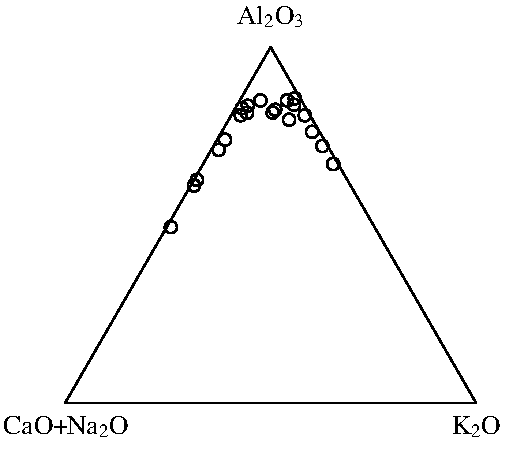
\includegraphics[width=\textwidth]{../figures/ACNK.pdf}\medskip
\end{minipage}
\begin{minipage}[t][][t]{.6\textwidth}
  \captionof{figure}{The A--CN--K diagram is a widely used graphical
    device in chemical weathering studies. It is a ternary diagram of
    Al\textsubscript{2}O\textsubscript{3}, CaO + Na\textsubscript{2}O
    and K\textsubscript{2}O, where the CaO refers to the silicate
    component of the sediment only (ignoring carbonates).  The
    composition on the diagram results from the competing effects of
    initial starting composition and chemical weathering. With
    increasing weathering intensity, A--CN--K compositions get pulled
    towards the Al\textsubscript{2}O\textsubscript{3} apex of the
    ternary diagram. This figure shows a synthetic dataset of 20
    A--CN--K measurements that have been affected by variable
    weathering intensities.\medskip}
  \label{fig:ACNK}
\end{minipage}

To obtain an average composition for the 20 samples, our natural
instinct is to calculate the arithmetic mean of their A--CN--K values:
\[
\begin{split}
  &\overline{\mbox{Al}_2\mbox{O}_3} =
  \sum\limits_{i=1}^{20} (\mbox{Al}_2\mbox{O}_3)_i/20 = 0.763 \\
  &\overline{\mbox{CaO} + \mbox{Na}_2\mbox{O}} =
  \sum\limits_{i=1}^{20} (\mbox{CaO}_2+\mbox{Na}_2\mbox{O})_i/20 = 0.141 \\
  &\overline{\mbox{K}_2\mbox{O}} =
  \sum\limits_{i=1}^{20} (\mbox{K}_2\mbox{O})_i/20 = 0.096
\end{split}
\]

Plotting this result on the ternary diagram reveals that it is
physically meaningless:

\noindent\begin{minipage}[t][][b]{.4\textwidth}
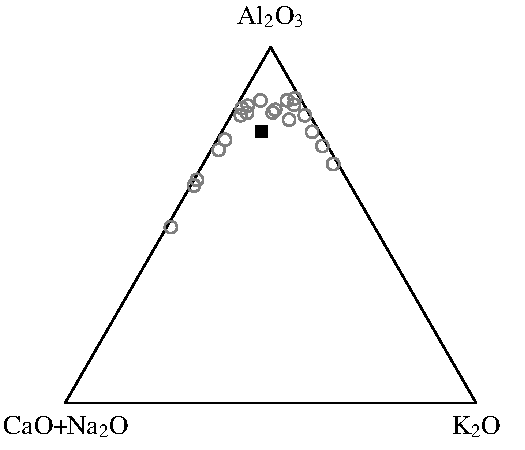
\includegraphics[width=\textwidth]{../figures/ACNKarithmeticmean.pdf}\medskip
\end{minipage}
\begin{minipage}[t][][t]{.6\textwidth}
  \captionof{figure}{ The black square represents the average A--CN--K
    composition of the 20 samples of Figure~\ref{fig:ACNK}. It is
    obtained by taking the arithmetic mean of all the
    Al\textsubscript{2}O\textsubscript{3}, (CaO +
    Na\textsubscript{2}O) and K\textsubscript{2}O concentrations using
    Equation~\ref{eq:mean}, and plotting the resulting 3-element
    vector as a new sample. This average composition plots outside the
    sample cloud, which is a meaningless result not unlike the porosity
    example of Figure~\ref{fig:porositylocation}.a.\medskip}
  \label{fig:ACNKarithmeticmean}
\end{minipage}

To quantify the dispersion of the data, we might be tempted to
calculate the standard deviation of the A--CN--K values:
\[
\begin{split}
  &s[\mbox{Al}_2\mbox{O}_3] =
  \sqrt{\sum\limits_{i=1}^{20}
    \frac{\left[(\mbox{Al}_2\mbox{O}_3)_i - 0.763\right]^2}{19}} = 0.0975 \\
  &s[\mbox{CaO} + \mbox{Na}_2\mbox{O}] =
  \sqrt{\sum\limits_{i=1}^{20}
    \frac{\left[(\mbox{CaO}_2+\mbox{Na}_2\mbox{O})_i - 0.141\right]^2}{19} } = 0.142 \\
  &s[\mbox{K}_2\mbox{O}] =
  \sqrt{\sum\limits_{i=1}^{20}
    \frac{\left[(\mbox{K}_2\mbox{O})_i - 0.096\right]^2}{19}} = 0.0926
\end{split}
\]

\noindent then we would expect $\sim$95\% of the data to fall into a
`2-sigma' interval around the mean
(Section~\ref{sec:normalproperties}):
\[
\begin{split}
  &\mbox{Al}_2\mbox{O}_3: 0.763 \pm 0.195 \\
  &\mbox{CaO} + \mbox{Na}_2\mbox{O}: 0.141 \pm 0.284 \\
  &\mbox{K}_2\mbox{O}: 0.096 \pm 0.185
\end{split}
\]

Note how the lower limits of the confidence regions for (CaO +
Na\textsubscript{2}O) and K\textsubscript{2}O have physically
impossible negative values. Visualising these limits as a 2-sigma
`confidence polygon':

\noindent\begin{minipage}[t][][b]{.4\textwidth}
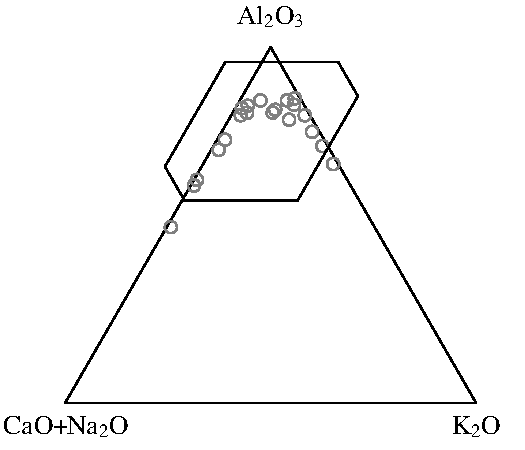
\includegraphics[width=\textwidth]{../figures/ACNKnaive.pdf}\medskip
\end{minipage}
\begin{minipage}[t][][t]{.6\textwidth}
  \captionof{figure}{The polygon represents a `95\% confidence region'
    for the arithmetic mean of Figure~\ref{fig:ACNKarithmeticmean}. It
    is obtained by 1) calculating the standard deviations of the
    Al\textsubscript{2}O\textsubscript{3}, (CaO +
    Na\textsubscript{2}O) and K\textsubscript{2}O concentrations using
    Equation~\ref{eq:stdev}; 2) multiplying these values by two; and
    3) subtracting or adding these values to the arithmetic mean of
    Figure~\ref{fig:ACNKarithmeticmean}. The resulting `2-sigma'
    bounds plot outside the ternary diagram, in physically impossible
    negative data space.\medskip}
  \label{fig:ACNKnaive}
\end{minipage}

The synthetic example shows that even the simplest summary statistics
do not work as expected when applied to compositional data.  The same
is true for more advanced statistical operations that are based on the
normal distribution. This includes linear regression
(Section~\ref{sec:MLregression}), principal component analysis
(Section~\ref{sec:PCA}) and discriminant analysis
(Section~\ref{sec:LDA}). These problems had long been known to
geologists, but a comprehensive solution was not found until the
1980s, by Scottish statistician John Aitchison.\medskip

The solution to the compositional data conundrum is closely related to
the solution of the ratio averaging problem discussed in
Section~\ref{sec:ratios}. The trick is to map the $n$-dimensional
composition to an $(n-1)$-dimensional Euclidean space by means of an
\textbf{additive logratio transformation} (alr). For example, in the
ternary case, we can map the compositional variables $x$, $y$ and $z$
to two transformed variables $v$ and $w$:
\begin{equation}
  v = \ln\!\left[\frac{x}{z}\right] \mbox{,~} w =
  \ln\!\left[\frac{y}{z}\right]
  \label{eq:alr}
\end{equation}

After performing the statistical analysis of interest (e.g.,
calculating the mean or constructing a 95\% confidence region) on the
transformed data, the results can then be mapped back to compositional
space with the inverse logratio transformation. For the ternary case:
\begin{equation}
  x = \frac{\exp[v]}{\exp[v] + \exp[w] + 1} \mbox{,~}
  y = \frac{\exp[w]}{\exp[v] + \exp[w] + 1} \mbox{,~}
  z = \frac{1}{\exp[v] + \exp[w] + 1}
  \label{eq:inverse-logratio-transformation}
\end{equation}

Applying this method to the A--CN--K dataset:\medskip

\noindent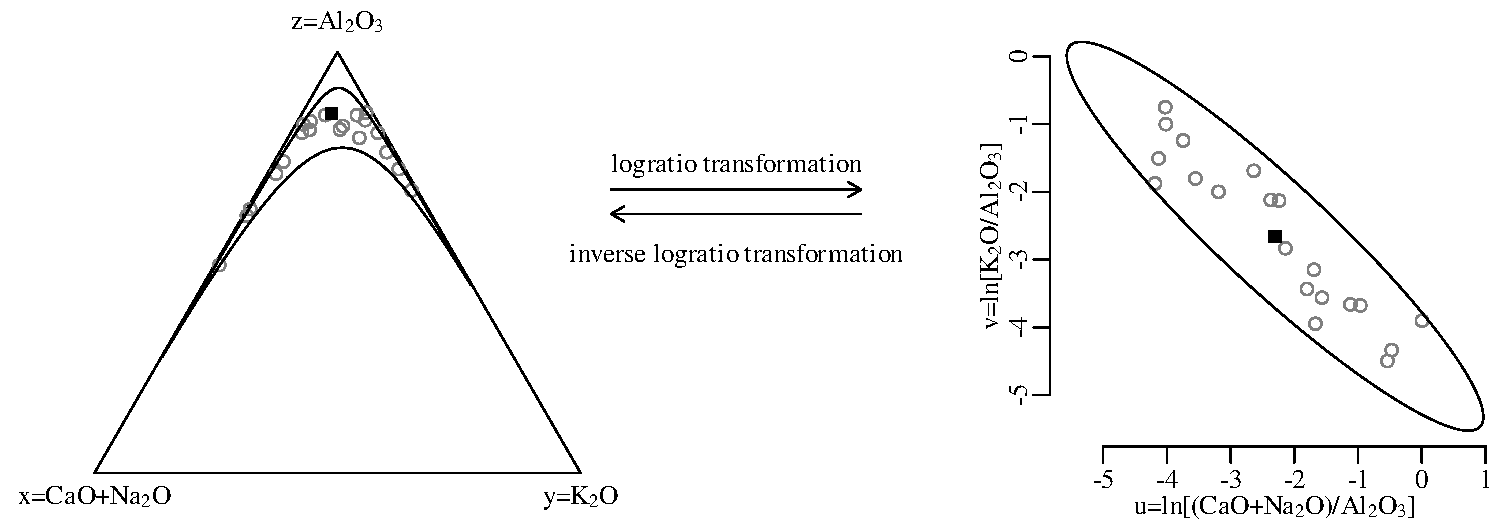
\includegraphics[width=\linewidth]{../figures/alr.PDF}
\begingroup \captionof{figure}{The additive logratio transformation
  (Equation~\ref{eq:alr}) maps data from an $n$-dimensional
  compositional space to an $(n-1)$-dimensional Euclidean space. For
  the A--CN--K data, it maps the data from a ternary diagram ($n=3$)
  to a bivariate ($n-1=2$) dataspace using Equation~\ref{eq:alr}. In
  this transformed space, it is safe to calculate the arithmetic mean
  (square) and confidence regions (ellipse). After completion of these
  calculations, the result can be mapped back to the ternary diagram
  using the inverse logratio transformation
  (Equation~\ref{eq:inverse-logratio-transformation}).\medskip}
\label{fig:alr}\endgroup

For the A--CN--K example, the transformed logratio mean plots inside
the heart of the data cloud. The 2-sigma confidence ellipse of the
logratios maps to a curved confidence region that entirely stays
within the ternary diagram and closely hugs the data. These results
are a lot more meaningful than the arithmetic mean and 2-sigma
confidence polygons of Figures~\ref{fig:ACNKarithmeticmean} and
\ref{fig:ACNKnaive}.\medskip

The logratio transformation makes intuitive sense. The very fact that
it is possible to plot a ternary diagram on a two-dimensional sheet of
paper already tells us that it really displays only two and not three
dimensions worth of information. The bivariate logratio variables more
faithfully represent the true information content of the compositional
data. The logratio transformation can easily be generalised from three
to more variables. For example, four-component compositional datasets
are constrained within a three dimensional triangle or tetrahaedron.
The general mathematical term for a constrained dataspace like a
ternary diagram or tetrahaedron is the \textbf{simplex}.  The additive
logratio transformation maps data from the simplex to an ordinary
Euclidean data space.

\section{PCA of compositional data}
\label{sec:compositionalPCA}

Table~\ref{tab:Major} shows the concentration of 10 major oxides in 16
samples of dune sand from the Namib sand sea:

\begin{center}
\begin{tabular}{c|cccccccccc}
 & SiO\textsubscript{2} & Al\textsubscript{2}O\textsubscript{3} & 
Fe\textsubscript{2}O\textsubscript{3} & MgO & CaO & Na\textsubscript{2}O & 
K\textsubscript{2}O & TiO\textsubscript{2} & 
P\textsubscript{2}O\textsubscript{5} & MnO\\ \hline
N1 & 82.54 & 6.14 & 3.18 & 1.65 & 2.24 & 1.16 & 1.35 & 0.44 & 0.11 & 0.06\\
N2 & 83.60 & 6.42 & 2.55 & 1.25 & 1.83 & 1.21 & 1.48 & 0.36 & 0.08 & 0.04\\
$\vdots$ & $\vdots$ & $\vdots$ & $\vdots$ & $\vdots$ & $\vdots$ &
$\vdots$ & $\vdots$ & $\vdots$ & $\vdots$ & $\vdots$ \\
N13 & 79.96 & 6.41 & 3.19 & 1.31 & 2.10 & 1.09 & 1.62 & 0.51 & 0.06 & 0.05\\
N14 & 73.62 & 9.96 & 4.07 & 2.01 & 3.45 & 1.86 & 2.29 & 0.44 & 0.10 & 0.07\\
T8 & 85.70 & 5.89 & 1.82 & 0.81 & 1.44 & 1.12 & 1.67 & 0.23 & 0.07 & 0.03\\
T13 & 82.54 & 6.02 & 2.30 & 1.42 & 3.07 & 1.19 & 1.46 & 0.34 & 0.11 & 0.04
\end{tabular}
\captionof{table}{The major element composition (in weight percent) of
  16 samples of Namib dune sand.}
\label{tab:Major}
\end{center}

It is not possible to plot this multivariate dataset on a single
two-dimensional diagram. Section~\ref{sec:PCA} introduced principal
component analysis as an effective way to address this issue by
projecting the data onto a two-dimensional subspace. Unfortunately we
cannot directly apply PCA to compositional data. For example, the
first step in the PCA analysis involves the calculation of an
arithmetic mean (Equation~\ref{eq:XMY}). However,
Section~\ref{sec:logratios} showed that the arithmetic mean of
compositional data can produce nonsensical results. This Section will
show that this problem can be solved using logratio
transformations.\medskip

Before we apply PCA to the data of Table~\ref{tab:Major}, let us first
illustrate the logratio solution using a simple toy example, which is
similar to the toy example that was used in
Section~\ref{sec:PCA}. Consider the following trivariate ($a$, $b$ and
$c$) dataset of three (1, 2 and 3) compositions that are constrained
to a constant sum ($a_i+b_i+c_i=100\%$ for $1\leq{i}\leq{3}$):
\begin{equation}
  X =
  \bbordermatrix{ & a & b & c \cr
   1 & 0.034 & 99.88 & 0.091 \cr
   2 & 69.45 & 25.55 & 5.01 \cr
   3 & 72.44 & 26.65 & 0.92
  }
  \label{eq:Xcomp}
\end{equation}

Plot the data on a ternary diagram:

\noindent\begin{minipage}[t][][b]{.3\textwidth}
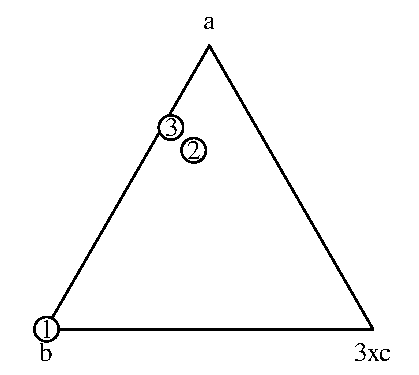
\includegraphics[width=\textwidth]{../figures/abc.pdf}\medskip
\end{minipage}
\begin{minipage}[t][][t]{.7\textwidth}
  \captionof{figure}{Ternary diagram of the synthetic toy example of
    Equation~\ref{eq:Xcomp}. Component $c$ has been multiplied by a
    factor of three to avoid an unsightly overlap between the plot
    symbols of samples 2 and 3, whose compositions are very
    similar.\medskip}
  \label{fig:abc}
\end{minipage}

Although the alr-transformation solves the closure problem, it is not
suitable for PCA because the axes of alr-coordinate spaces are not
orthogonal to each other:

\noindent\begin{minipage}[t][][b]{.3\textwidth}
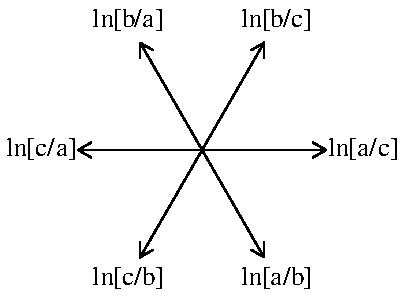
\includegraphics[width=\textwidth]{../figures/alraxes.pdf}\medskip
\end{minipage}
\begin{minipage}[t][][t]{.7\textwidth}
  \captionof{figure}{There are six different ways to form logratios in
    the ternary data space. These six logratios define three
    coordinate axes that intersect each other at 60$^\circ$ angles. As
    a consequence, distances in alr-space depend on the choice of
    logratios.\medskip}
  \label{fig:alraxes}
\end{minipage}

For example, calculate the distance between the alr-coordinates of
samples~2 and 3 of Equation~\ref{eq:Xcomp}, first using $b$ as a
common denominator ($d[2,3]_b$), and then using $c$ as a common
denominator ($d[2,3]_c$):
\begin{equation*}
  \begin{split}
    d[2,3]_b & =
    \sqrt{
      \left(
      \ln\!\left[\frac{69.45}{25.55}\right]-
      \ln\!\left[\frac{72.44}{26.65}\right]
      \right)^2 +
      \left(
      \ln\!\left[\frac{5.01}{25.55}\right]-
      \ln\!\left[\frac{0.92}{26.65}\right]
      \right)^2
    } = 1.74\\
    & \neq 
    \sqrt{
      \left(
      \ln\!\left[\frac{69.45}{5.01}\right]-
      \ln\!\left[\frac{72.44}{0.92}\right]
      \right)^2 +
      \left(
      \ln\!\left[\frac{25.55}{5.01}\right]-
      \ln\!\left[\frac{26.65}{0.92}\right]
      \right)^2
    } = 2.46 = d[2,3]_c
  \end{split}
\end{equation*}

The fact that distances are not unequivocally defined in alr-space
spells trouble for PCA. Recall the equivalence of PCA and classical
MDS, which was discussed in Section~\ref{sec:MDS}. MDS is based on
dissimilarity matrices, and so if distances are not well defined, then
neither are the MDS configuration and, hence, the principal
components. This issue can be solved by using a different type of
logratio transformation, the \textbf{centred logratio transformation}
(clr):
\begin{equation}
  u_i = \ln\!\left[\frac{x_i}{g_i}\right] \mbox{,~}
  v_i = \ln\!\left[\frac{y_i}{g_i}\right] \mbox{,~and~}
  w_i = \ln\!\left[\frac{z_i}{g_i}\right]
  \label{eq:clr}
\end{equation}

\noindent where $g_i$ is the geometric mean of the
$i$\textsuperscript{th} sample:
\[
g_i = \exp\!\left[\frac{\ln[x_i]+\ln[y_i]+\ln[z_i]}{3}\right]
\]

Unlike alr-coordinate axes, clr-coordinate axes are orthogonal and
unequivocally define a set of well behaved distances. Applying the
clr-transformation to the data of Equation~\ref{eq:Xcomp} yields a new
trivariate dataset:
\begin{equation}
  X\textsubscript{c} =
  \bbordermatrix{ & \ln(a/g) & \ln(b/g) & \ln(c/g) \cr
    1 & -3 & 5 & -2 \cr
    2 & 1.21  & 0.21 & -1.42 \cr
    3 & 1.79  & 0.79 & -2.58
  }
  \label{eq:Xc}
\end{equation}


\noindent where $g$ stands for the geometric mean of each row. Note
that each of the rows of $X_c$ adds up to zero. Thanks to the symmetry
of the clr-coordinates, whose three-dimensional axes are perpendicular
to each other, the distances between the rows (which are also known as
\textbf{Aitchison distances}) are well defined. Subjecting
Equation~\ref{eq:Xc} to the same matrix decompositions as
Equations~\ref{eq:XMY}--\ref{eq:P} yields:
\begin{align}
  \begin{split}
    X_c & = 1_{3,1}~M + P~Q^{-1} \\
    ~ & = 
    \left[
      \begin{array}{c}
        1 \\
        1 \\
        1
      \end{array}
      \right]
   \left[
    \begin{array}{ccc}
        0 & 2 & -2
      \end{array}
      \right]
    + 
     \left[
      \begin{array}{ccc}
        -4.24 &  0   & 0 \\
        2.12  & -7.1 & 0 \\
        2.12  &  7.1 & 0
      \end{array}
      \right]
    \left[
      \begin{array}{ccc}
        0.71 & -0.71 &  0 \\
        0.41 &  0.41 & -0.82 \\
        0.58 &  0.58 &  0.58
      \end{array}
      \right]
    \label{eq:PCAcomp}
  \end{split}
\end{align}

Note that, even though this yields three principal components instead
two, the scores of the third component in matrix $P$ are all zero.
Therefore, all the information is contained in the first two
components\footnote{The covariance matrix of $X_c$ is singular and
therefore the third eigenvalue is zero as well.}. Also note that the
first two principal components of the compositional dataset are
identical to those of the PCA example shown in
Equation~\ref{eq:P}. This is, of course, intentional:

\noindent\begin{minipage}[t][][b]{.32\textwidth}
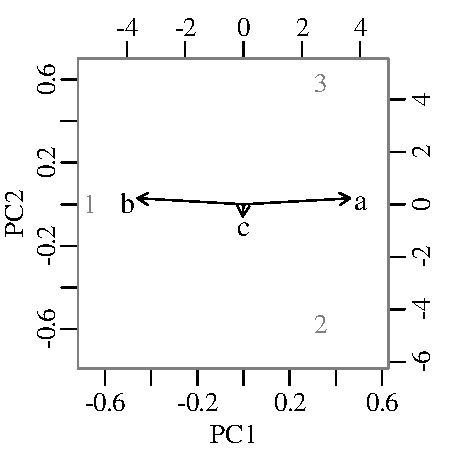
\includegraphics[width=\textwidth]{../figures/clrPCA.pdf}\medskip
\end{minipage}
\begin{minipage}[t][][t]{.68\textwidth}
  \captionof{figure}{Compositional biplot of the toy data using the
    clr transformation. The biplot tells us that sample~1 is rich in
    component $b$, whereas samples~2 and 3 are rich in component
    $a$. The difference between samples~2 and 3 is due to a small
    difference in component $c$.  Compare with the ternary diagram
    (Figure~\ref{fig:abc}) to verify these conclusions.\medskip}
  \label{fig:clrPCA}
\end{minipage}

Applying the same procedure to the Namib dataset of
Table~\ref{tab:Major}:

\noindent\begin{minipage}[t][][b]{.4\textwidth}
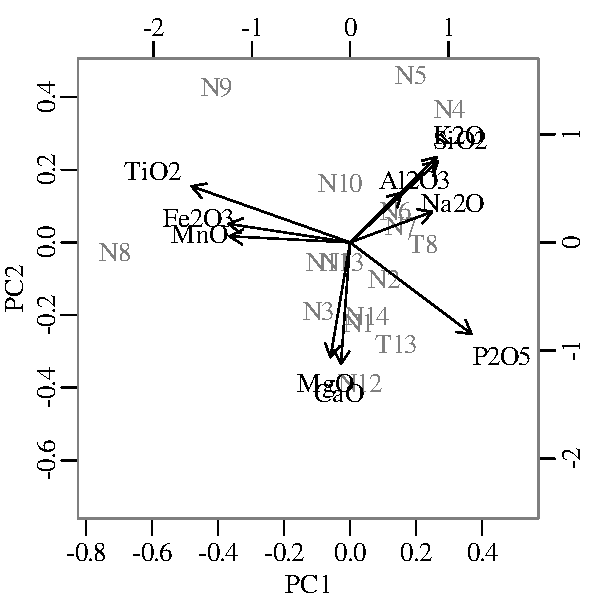
\includegraphics[width=\textwidth]{../figures/majorPCA.pdf}\medskip
\end{minipage}
\begin{minipage}[t][][t]{.6\textwidth}
  \captionof{figure}{Compositional biplot of the major element
    concentration data of Table~\ref{tab:Major}, with the samples
    shown in grey and the vector loadings in black. Samples that plot
    close together (such as N1 and N14) are compositionally similar,
    whereas samples that plot far apart (such as N8 and T8) are
    compositionally different. One should be careful not to interpret
    the individual rays of compositional biplots. For example, one
    cannot safely conclude that N8 is enriched in MnO relative to
    T8. However, it is safe to say that N8 has a higher
    MnO/Na\textsubscript{2}O-ratio than T8. \medskip}
  \label{fig:majorPCA}
\end{minipage}

With regard to the rays, the key information is contained in the
\textbf{links} between them. For example, the link between MgO and CaO
on Figure~\ref{fig:majorPCA} is short, which suggests that these two
oxides are proportional and their (log)ratios exhibit little
scatter. In contrast, the link between K\textsubscript{2}O and MgO is
long, so their logratios are more dispersed. The link between
TiO\textsubscript{2} and CaO is collinear with that between MnO and
MgO. This indicates that the TiO\textsubscript{2} -- CaO -- MnO -- MgO
\textbf{subcomposition} forms a one dimensional pattern. The link
between K\textsubscript{2}O and CaO is perpendicular to that between
TiO\textsubscript{2} and P\textsubscript{2}O\textsubscript{5},
suggesting that the corresponding subcompositions are independent:
\begin{center}
\noindent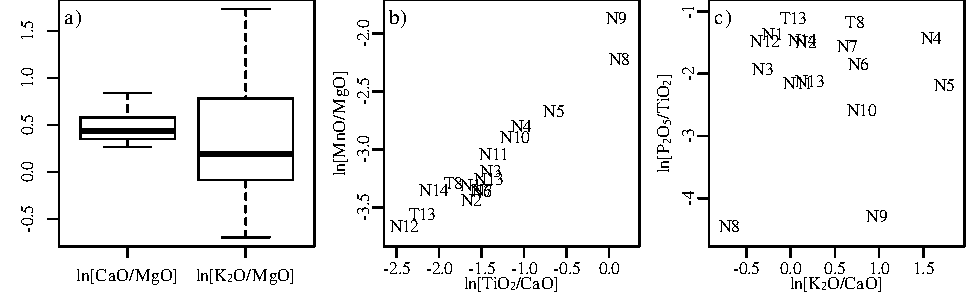
\includegraphics[width=.95\textwidth]{../figures/links.pdf}
\captionof{figure}{Subcompositional analysis of
  Figure~\ref{fig:majorPCA}. a) Box plots of the CaO/MgO-logratio
  (short link) and the K\textsubscript{2}O/MgO-logratio (long link);
  b) The collinearity of the links between TiO\textsubscript{2}, CaO,
  MnO and MgO indicates strong correlation of the samples in
  ln[MnO/MgO] -- ln[TiO\textsubscript{2}/CaO] space; c) The link
  between P\textsubscript{2}O\textsubscript{5} and
  TiO\textsubscript{2} is orthogonal to that between between
  K\textsubscript{2}O and CaO, reflecting independence of the
  corresponding logratios.}
  \label{fig:links}
\end{center}

Although the alr and clr transformations act in slightly different
ways, they both achieve the same effect, namely to `liberate' the
compositional data from the confines of the simplex and map it to a
Euclidean space in which values are free to take any value from
$-\infty$ to $+\infty$. Logratio transformations allow compositional
data to be analysed by a host of standard statistical techniques,
including not only PCA, but also clustering and discriminant analysis.

\section{LDA of compositional data}
\label{sec:compositionalLDA}

Section~\ref{sec:compositionalPCA} showed how we can safely apply
unsupervised learning techniques such as PCA to compositional data
after performing a logratio transformation. Exactly the same procedure
can be applied to supervised learning techniques such as LDA. We will
illustrate this with an example from igneous petrology:

\noindent\begin{minipage}[t][][b]{.35\textwidth}
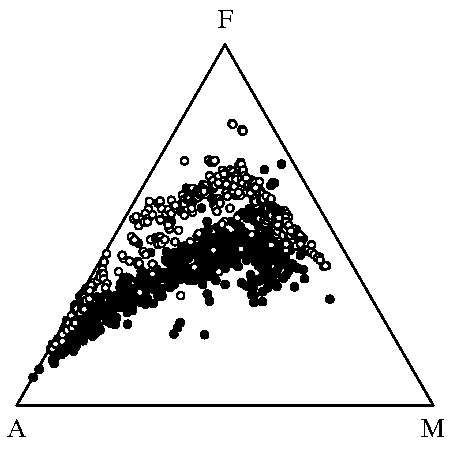
\includegraphics[width=\textwidth]{../figures/AFM.pdf}\medskip
\end{minipage}
\begin{minipage}[t][][t]{.65\textwidth}
  \captionof{figure}{A dataset of igneous rock compositions from
    Iceland and the Cascades Mountains on a ternary A--F--M diagram
    (where A = Na\textsubscript{2}O+K\textsubscript{2}O, F =
    Fe\textsubscript{2}O\textsubscript{3}+FeO and M = MgO). The white
    dots define a `Fenner' trend marking the tholeiitic suite of
    igneous rocks from Iceland. The black dots define a `Bowen' trend,
    marking the calc-alkaline suite of rocks from the Cascades.\medskip}
  \label{fig:AFM}
\end{minipage}

Plotting the same data in logratio space:

\noindent\begin{minipage}[t][][b]{.35\textwidth}
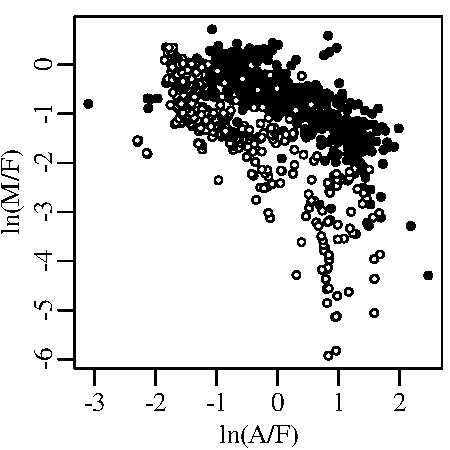
\includegraphics[width=\textwidth]{../figures/lrAFM.pdf}\medskip
\end{minipage}
\begin{minipage}[t][][t]{.65\textwidth}
  \captionof{figure}{The additive logratio transformation liberates
    the A--F--M data from the confines of the ternary diagram and maps
    them to a Euclidean dataspace in which logratios are free to take
    any value from $-\infty$ to $+\infty$. In this space, the ln(M/F)
    vs. ln(A/F) values of the tholeiitic and calc-alkali rock suites
    are clustered into two distinct clouds of roughly equal size that
    have all the hallmarks of bivariate normal distributions with a
    shared covariance matrix. Thus the transformed data seems well
    suited for linear discriminant analysis.\medskip}
  \label{fig:lrAFM}
\end{minipage}

Applying LDA to the A--F--M data and visualising the results in both
logratio space and the ternary diagram:

\noindent\begin{minipage}[t][][b]{.7\textwidth}
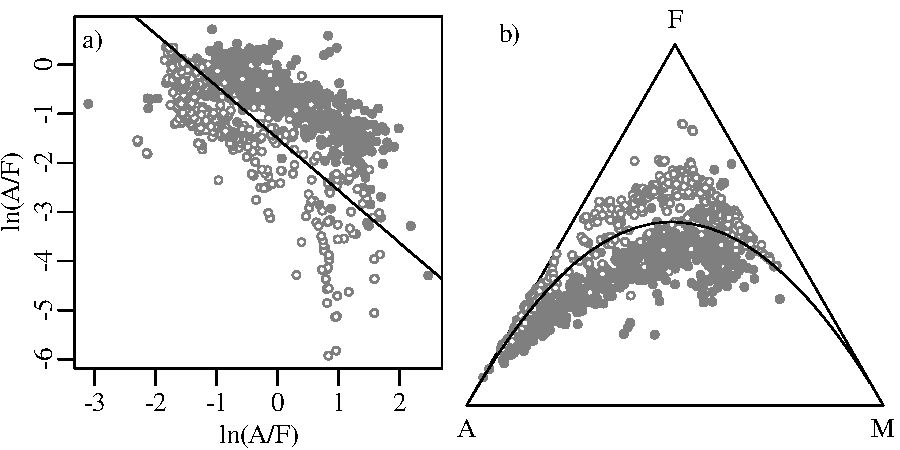
\includegraphics[width=\textwidth]{../figures/LDAAFM.pdf}\medskip
\end{minipage}
\begin{minipage}[t][][t]{.3\textwidth}
  \captionof{figure}{LDA of the A--F--M data shown in a) logratio
    space and b) a ternary diagram.\medskip}
  \label{fig:LDAAFM}
\end{minipage}

The linear boundary between the tholeiitic and calc-alkaline fields of
the A--F--M logratio diagram is not only an effective discriminator
between these two fields, but it also encodes some real geochemical
information about the petrogenesis of igneous
rocks. Section~\ref{sec:logratio-processes} will show how fundamental
compositional processes can lead to simple laws in logratio space.

\section{Logratio processes}
\label{sec:logratio-processes}

Consider a magma containing $A$ mass units of
Na\textsubscript{2}O+K\textsubscript{2}O, $F$ mass units of
FeO+Fe\textsubscript{2}O\textsubscript{3}, and $M$ mass units of
MgO. Suppose that, as the magma cools, it loses components $A$, $F$
and $M$ at rates that are proportional to the amounts of $A$, $F$ and
$M$ present in the magma:
\begin{equation}
  \frac{\partial A}{\partial t} = -\lambda_A A \mbox{,~}
  \frac{\partial F}{\partial t} = -\lambda_F F \mbox{,~and~}
  \frac{\partial M}{\partial t} = -\lambda_M M
  \label{eq:decay}
\end{equation}

\noindent where $t$ is time and $\lambda_x$ is a decay constant (for
$x \in \{A, F, M\}$). The same mathematical formulation can be used to
describe the settlement of sediment from a suspension, or the decay of
radioactive isotopes.  The solution to Equation~\ref{eq:decay} is a
set of exponential functions:
\begin{equation}
  A = A_\circ \exp(-\lambda_A t) \mbox{,~}
  F = F_\circ \exp(-\lambda_F t) \mbox{,~and~}
  M = M_\circ \exp(-\lambda_M t)
  \label{eq:expdecay}
\end{equation}

\noindent where $A_\circ$, $F_\circ$ and $M_\circ$ are the initial
values of $A$, $F$ and $M$ in the primitive magma. Different values of
$\lambda_A$, $\lambda_F$ and $\lambda_M$ give rise to different
trajectories on the AFM diagram. Combining the three compositional
variables $A$, $F$ and $M$ into two logratio variables $\ln(A/F)$ and
$\ln(M/F)$ recasts the exponential functions of
Equation~\ref{eq:expdecay} into two linear functions:
\begin{align}
  \ln(A/F) = & \ln(A_\circ/F_\circ) + (\lambda_F-\lambda_A)t\\
  \ln(M/F) = & \ln(M_\circ/F_\circ) + (\lambda_F-\lambda_M)t
\end{align}

\noindent which can be combined as follows:
\begin{equation}
  \begin{split}
    \ln(A/F) = & C_1 \ln(M/F) + C_2 \\
    \mbox{where~} C_1 = & \frac{\lambda_F-\lambda_A}{\lambda_F-\lambda_M} \\
    \mbox{and~} C_2 = & \ln(A_\circ/F_\circ) - C_1 \ln(M_\circ/F_\circ) 
  \end{split}
\end{equation}

Thus, the curved trajectories on the AFM diagram become straight lines
in logratio space. This is exactly the behaviour that was observed in
Figure~\ref{fig:LDAAFM}. Evaluating the compositional evolution of
three different A--F--M systems:

\begin{center}
\begin{tabular}{c|cccccc}
  & starting position & $\ln[A_\circ/F_\circ]$ & $\ln[M_\circ/F_\circ]$ &
  $\lambda_A$ & $\lambda_F$ & $\lambda_M$ \\ \hline
  1 & $i$ & -2 & 1 & 4 & 6 & 8 \\
  2 & $i$ & -2 & 1 & 4 & 7 & 8 \\
  3 & $ii$ & 1 & 2 & 4 & 4 & 8 \\
\end{tabular}
\end{center}
  
\noindent produces the following output:

\noindent\begin{minipage}[t][][b]{.7\textwidth}
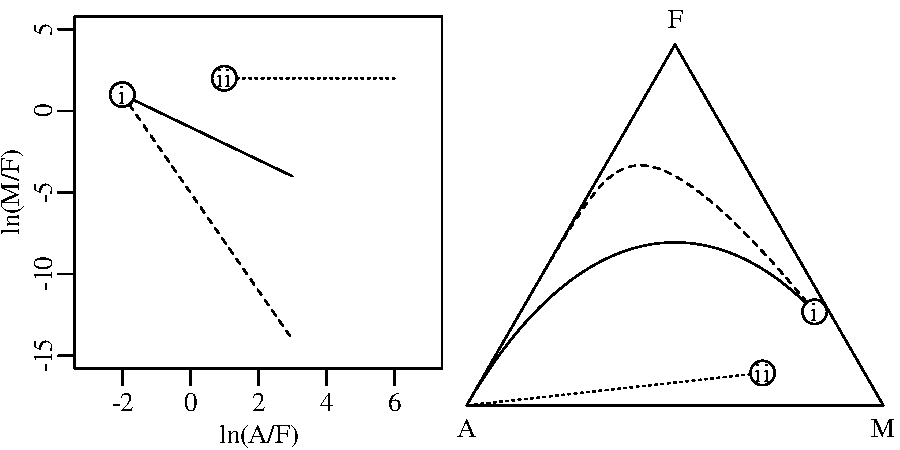
\includegraphics[width=\textwidth]{../figures/cath.pdf}\medskip
\end{minipage}
\begin{minipage}[t][][t]{.3\textwidth}
  \captionof{figure}{Exponential decay processes of compositional data
    become linear trends in logratio space. Initial composition $i$
    forms the starting point of two trajectories, marked by dashed and
    solid lines, respectively. These trends are characterised by
    different decay parameters.\medskip}
  \label{fig:cath}
\end{minipage}

The dashed and solid lines in Figure~\ref{fig:cath} mimic the Fenner
and Bowen trends of the tholeiitic and calc-alkaline magma series,
respectively. This makes geological sense because it is not hard to
imagine how $\lambda_F$ could depend on the oxygen fugacity in the
magma, which controls the valence state of the Fe-ions and, hence, the
minerals that they form.
